%!TEX root = ../index.tex

\section{Architecture}

browserCloud.js proposes a mechanism to find, gather and utilize idle resources through a P2P overlay network. Participants will be joining and connecting to each other through a rendezvous point, as represented in Figure~\ref{fig:b-e}. Any Peer that joins the network can submit a job which will be partitioned and distributed across peers available. Once a Peer completes its task, it is sends back the results to the issue. The user does not need to understand how the network is organized or which peers it is directly connected too, that complexity is abstracted by browserCloud.js.

\begin{figure}[h!]
  \centering
  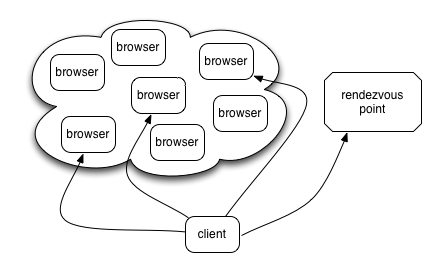
\includegraphics[width=0.35\textwidth]{figs/birds-eye}
  \caption{browserCloud.js Overview}
  \label{fig:b-e}
\end{figure}

A pratical use case for browserCloud.js is high CPU bound jobs that can run in parallel, e.g: image processing, video compressing, data manipulation, map and reduce tasks, etc. These parallel tasks are divided by the peers available in the network, leveraging the parallelism to obtain a speed up.

browserCloud.js was architectured to meet the following requirements:

\begin{itemize}
    \item \textbf{Membership management} - The system has to enable peers to join and leave a current network of browserCloud.js peers or a subset of it.
    \item \textbf{Message routing} - Messages are be routed between peers, having each peer knowing a subset of the network, guaranteeing in full coverage in this manner.
    \item \textbf{Job scheduling and results aggregation} - The discovery of computational resources must be performed using a distributed approach, peers interact between each other to send tasks and retrieve the results for the peer executing the job.
    \item \textbf{Support dynamic runtime} - Provide flexibility for jobs being executed. 
    \item \textbf{Reduced entrance cost to enable greater adoption} - Simple APIs design, abstracting the complexity in favor of greater extendability.
    \item \textbf{Enable integration and compliance tests} - Automate the process of verifying browserCloudjs integrity and functionality.
\end{itemize}

\subsection{Distributed Architecture}

The overview of the distributed architecture can be seen in Figure~\ref{fig:n-a-o}.

\begin{figure}[h!]
  \centering
  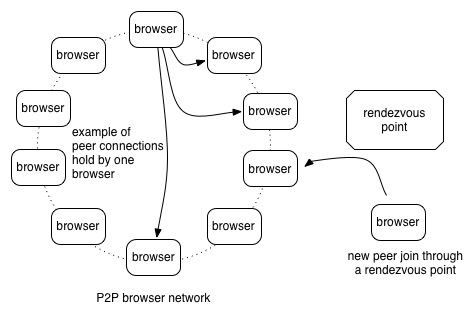
\includegraphics[width=0.35\textwidth]{figs/network-architecture-overview}
  \caption{browserCloud.js Distributed Architecture Overview}
  \label{fig:n-a-o}
\end{figure}

\subsubsection{Entities}

There are two different kind of actors in the system:

\begin{itemize}
    \item browser - The points on our network that will be able to issue jobs, execute tasks and route messages.
    \item rendezvous point - The only centralized component in this architecture, its purpose is for the clients to have a way to connect to and join the overlay network.
\end{itemize}

\subsubsection{Interaction Protocols}

In a browserCloud.js infrastructure, we have three main interaction patterns. The first being when a peer joins or leaves the network, membership management. In traditional P2P network, we could simply exchange IP:Port pairs, but in a P2P browser network, a RTCPeerConnection has to be established and kept alive, meaning that an handshaking protocol must be performed. The second pattern is message routing between peers, this has been designed with inspiration on the Chord\cite{Stoica2001},routing algorithm, studied on the related work. The third interaction demonstrates how to levarage the computer cycles available in the network to process CPU bound jobs.

\paragraph{Peer joins and leaves}

A peer join compromisses of the following steps:

\begin{itemize}
    \item \textbf{1 - Registration} - When a peer is ready to join the network, it performs the registration action to the custom browserCloud.js signalling server, the server replies with a confirmation and a unique ID for this peer to occupy in the network. This enables the signalling server, which holds the meta data of the current state in the network, to pick the ID in the ID interval that might be less occupied. We can observe this interaction in Figure~\ref{fig:1-p-r}.
    \item \textbf{2 - New peer available} - As peers join the network, the other peers get notified to establish or update their routing tables, keeping the message routing efficient (explained in the next subsection). For each peer join, a notification with a finger update can be sent to 1 or more peers present, as seen in Figure~\ref{fig:2-p-n}.
    \item \textbf{3 - Connection establishment between two peers} - In order to establish a connection between two peers, once there is an interest for these to connect, for e.g, in the case of a finger update event. There are two substeps, the first being the SDP offer creation through a step called "hole punching". A browser uses the WebRTC APIs to traverse through NAT to obtain its public IP, which is crucial information when two browsers need to establish a direction connection, Figure~\ref{fig:3-p-s}. The second step is the exchange of these SDP offers between browsers and that has to be performed by a centralized service; in browserCloud.js we developed a custom signalling server that handles that part, as seen in Figure~\ref{fig:4-p-c}.
\end{itemize}

A peer leave is a simpler and organic process, once a peer leaves the network, the RTCPeerConnections objects are closed and destroyed, notifying automatically the peers that have to update their routing tables.

\begin{figure}[h!]
  \centering
  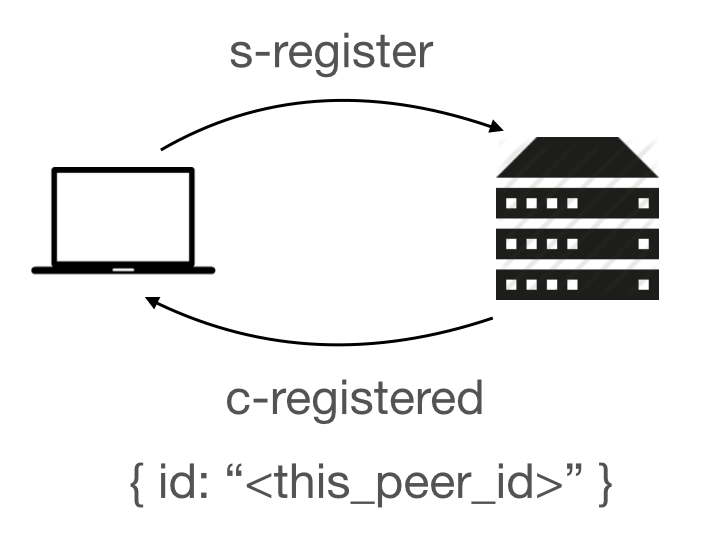
\includegraphics[width=0.2\textwidth]{figs/1-peer-registers}
  \caption{Registration of a peer, signaling itself as available to be part of the P2P network}
  \label{fig:1-p-r}
\end{figure}

\begin{figure}[h!]
  \centering
  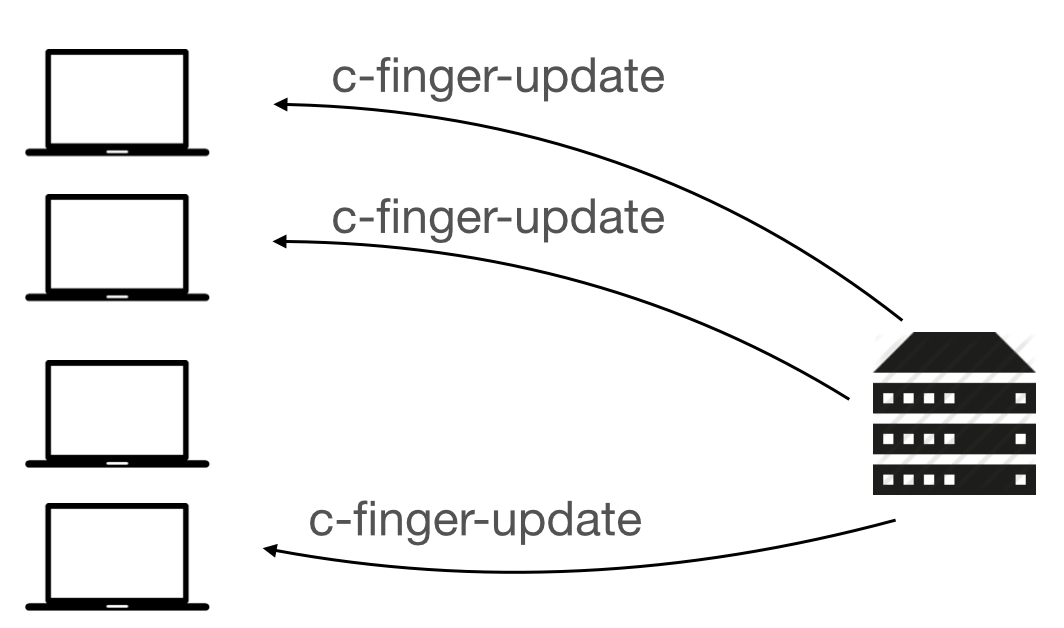
\includegraphics[width=0.2\textwidth]{figs/2-peers-notified}
  \caption{A peer is notified to update his finger table}
  \label{fig:2-p-n}
\end{figure}

\begin{figure}[h!]
  \centering
  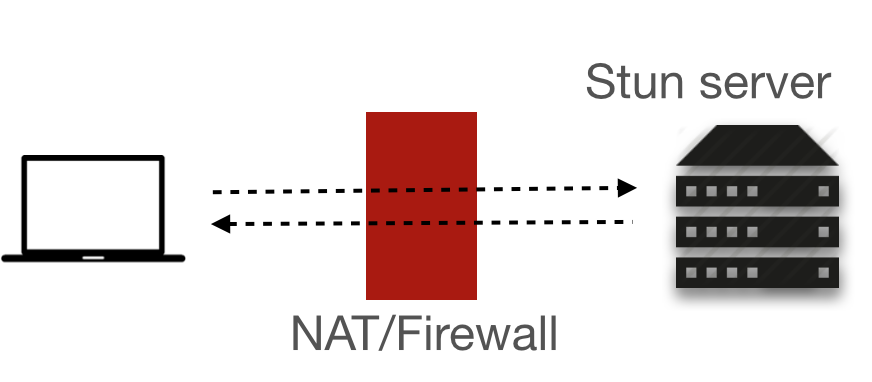
\includegraphics[width=0.2\textwidth]{figs/3-peer-stun}
  \caption{Hole punching through NAT to obtain a public IP and create a SDP offer}
  \label{fig:3-p-s}
\end{figure}

\begin{figure}[h!]
  \centering
  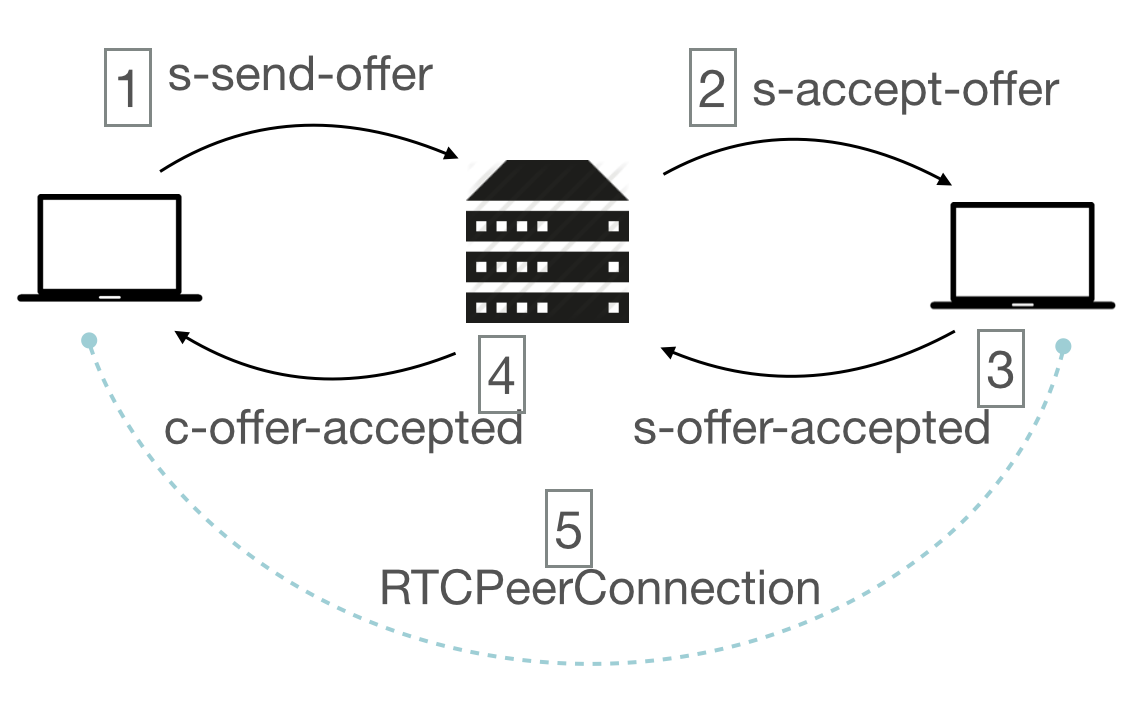
\includegraphics[width=0.2\textwidth]{figs/4-peer-connect}
  \caption{Establishment of a RTCPeerConnection through the custom Signalling Server}
  \label{fig:4-p-c}
\end{figure}

\paragraph{Message routing}

For message routing, we designed an adaptation of the Chord routing algorithm, a P2P Structured Overlay network, a DHT studied in the related work, with the goal of keeping an efficient routing and resource lookup with the increase of the number of peers in the network.

The ID namespace available in our DHT consists of 48 bit IDs (Figure~\ref{fig:c-1} ), this decision was made due to the fact that Javascript only supports 53 bit numbers, to support a greater variaty of IDs, we would have to resort to a big integer third party library, adding unnecessary consuption of computing resources. However, for demonstration purposes, we will explain using a 3 bit ID namespace.

\begin{figure}[h!]
  \centering
  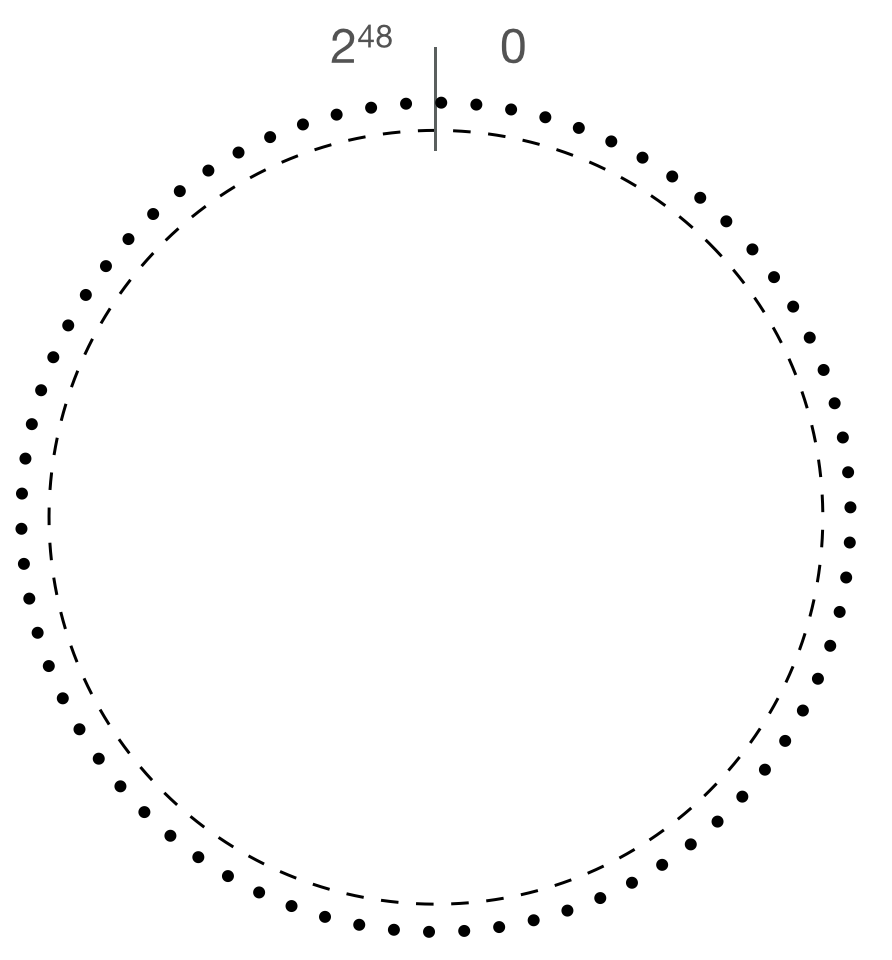
\includegraphics[width=0.2\textwidth]{figs/chord-1}
  \caption{How the ID namespace is visualized in the DHT}
  \label{fig:c-1}
\end{figure}

In Figure~\ref{fig:c-2}, we have a DHT composed of 4 different peers, with IDs 0, 1, 3 and 6. Each one of these peers will be responsible for a segment of the DHT, in another words what this means is that every message that is destined to their segment, will be delivered to respective peer responsable. A peer is responsible for a segment of IDs greater than the peer that is its predecessor and lesser or equal than its own ID, represented in Figure ~\ref{fig:c-3}. When a peer enters in the network, its ID is generated through a crop of a SHA-1 hash from a random generated number, creating a natural uniform distribution.

\begin{figure}[h!]
  \centering
  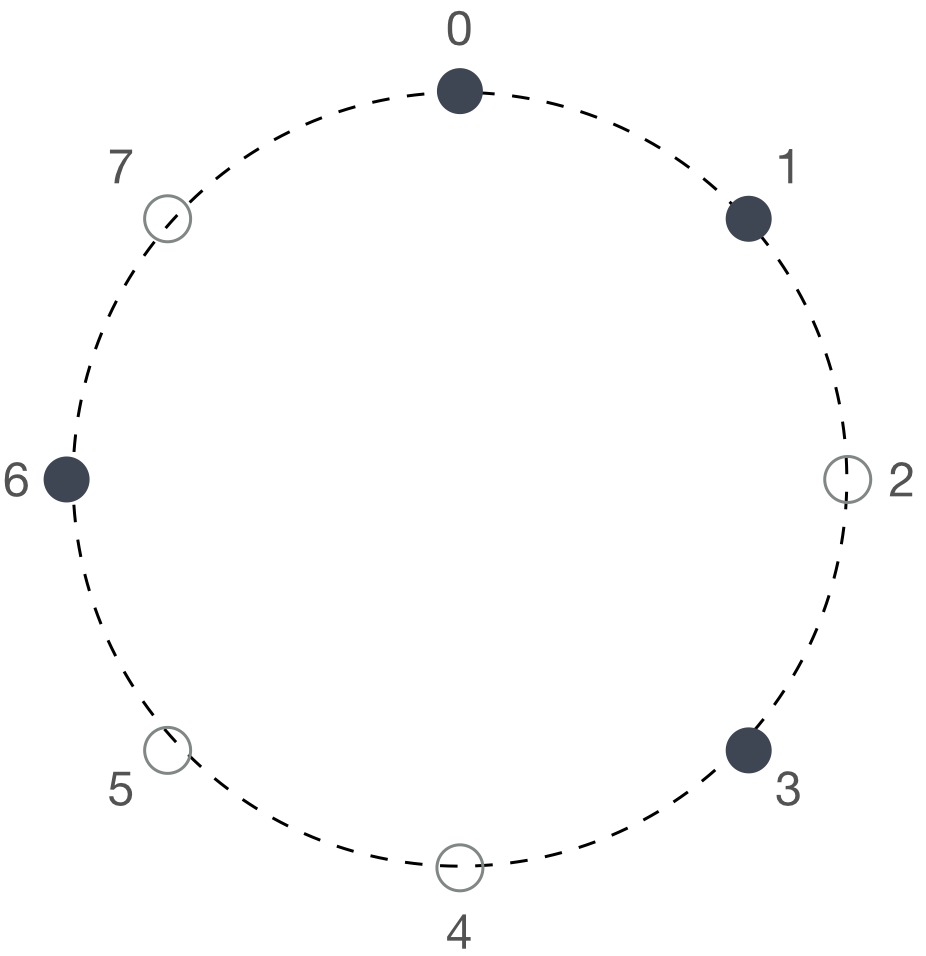
\includegraphics[width=0.2\textwidth]{figs/chord-2}
  \caption{Example of a DHT with 4 peers for case study}
  \label{fig:c-2}
\end{figure}

\begin{figure}[h!]
  \centering
  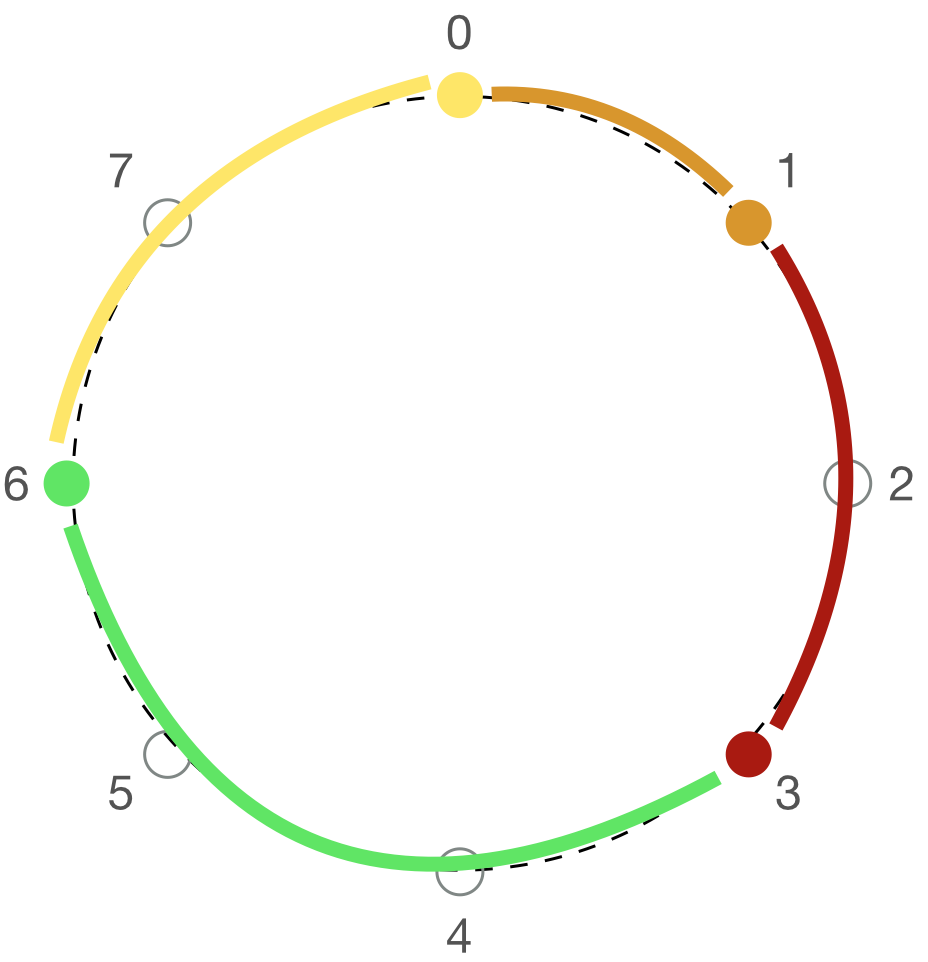
\includegraphics[width=0.2\textwidth]{figs/chord-3}
  \caption{Responsability interval for each Peer}
  \label{fig:c-3}
\end{figure}

In order for messages to find its correct destination, each peer has to know at minimum the peer that is next to it on the DHT, also called "successor" (Figure~\ref{fig:c-4}). Messages will be forward until they reach the peer which compromisses the responsability of being responsible for that message ID.

\begin{figure}[h!]
  \centering
  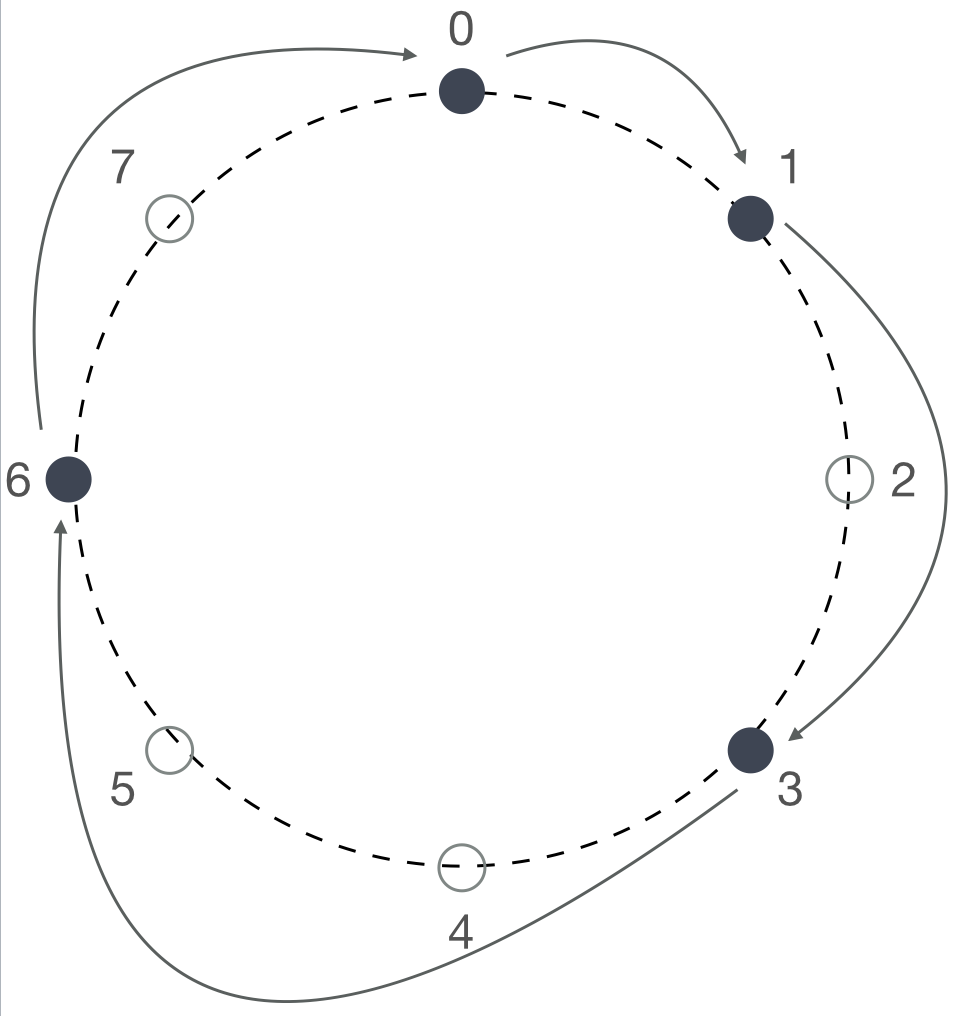
\includegraphics[width=0.2\textwidth]{figs/chord-4}
  \caption{Minimum number of connections for messages to be routed properly}
  \label{fig:c-4}
\end{figure}

However, as specified earlier in the document, we want to achieve a good and stable efficiency when it comes to routing messages inside the DHT as the network grows. To achieve that, we introduce fingers in our peers as we mentioned earlier. A finger is a direct connection to another peer in the network (Figure~\ref{fig:c-5}), that was picked following a specific distribution, each peer will have 1 to N fingers, where N is the number of bits of the IDs (for this example, N = 3). A finger is always the peer responsible for the "start" value of the interval (see Figure~\ref{fig:c-6} for reference and formula) and a message will be routed to that finger if it falls inside the interval.

\begin{figure}[h!]
  \centering
  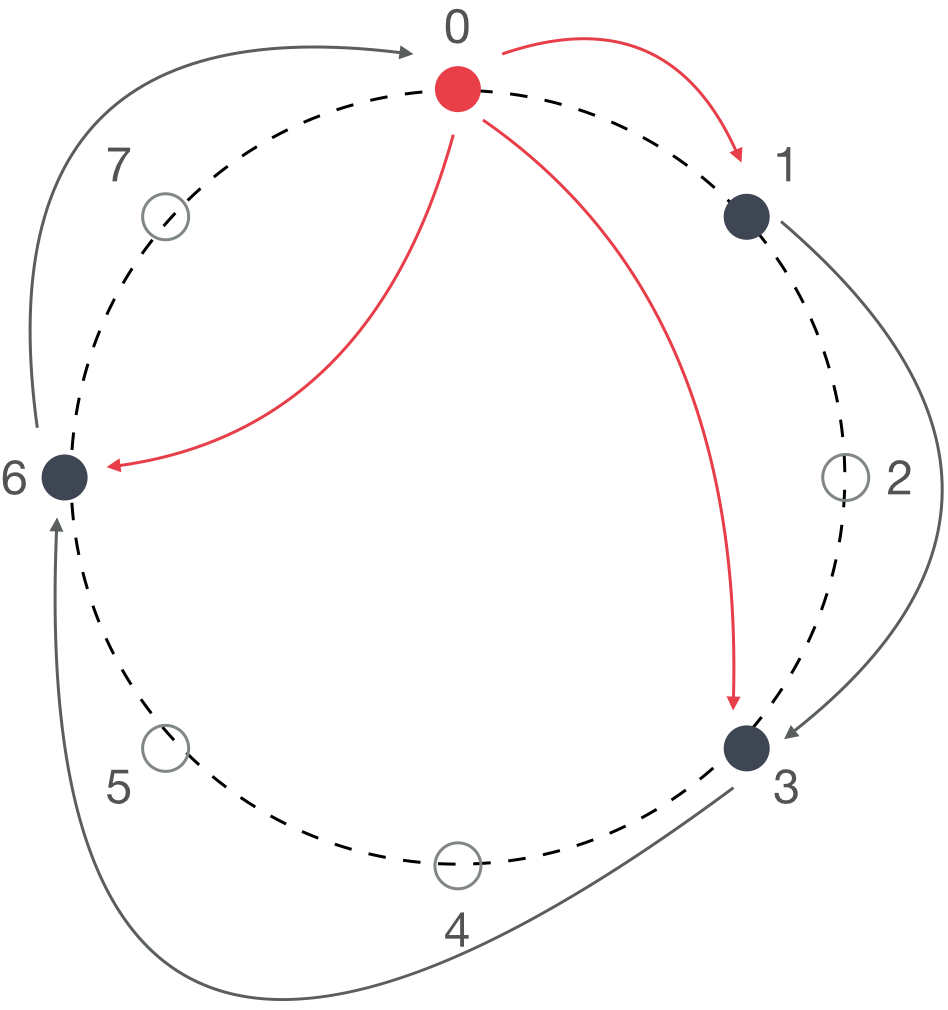
\includegraphics[width=0.2\textwidth]{figs/chord-5}
  \caption{Example of peer with ID = 0 fingers}
  \label{fig:c-5}
\end{figure}

\begin{figure}[h!]
  \centering
  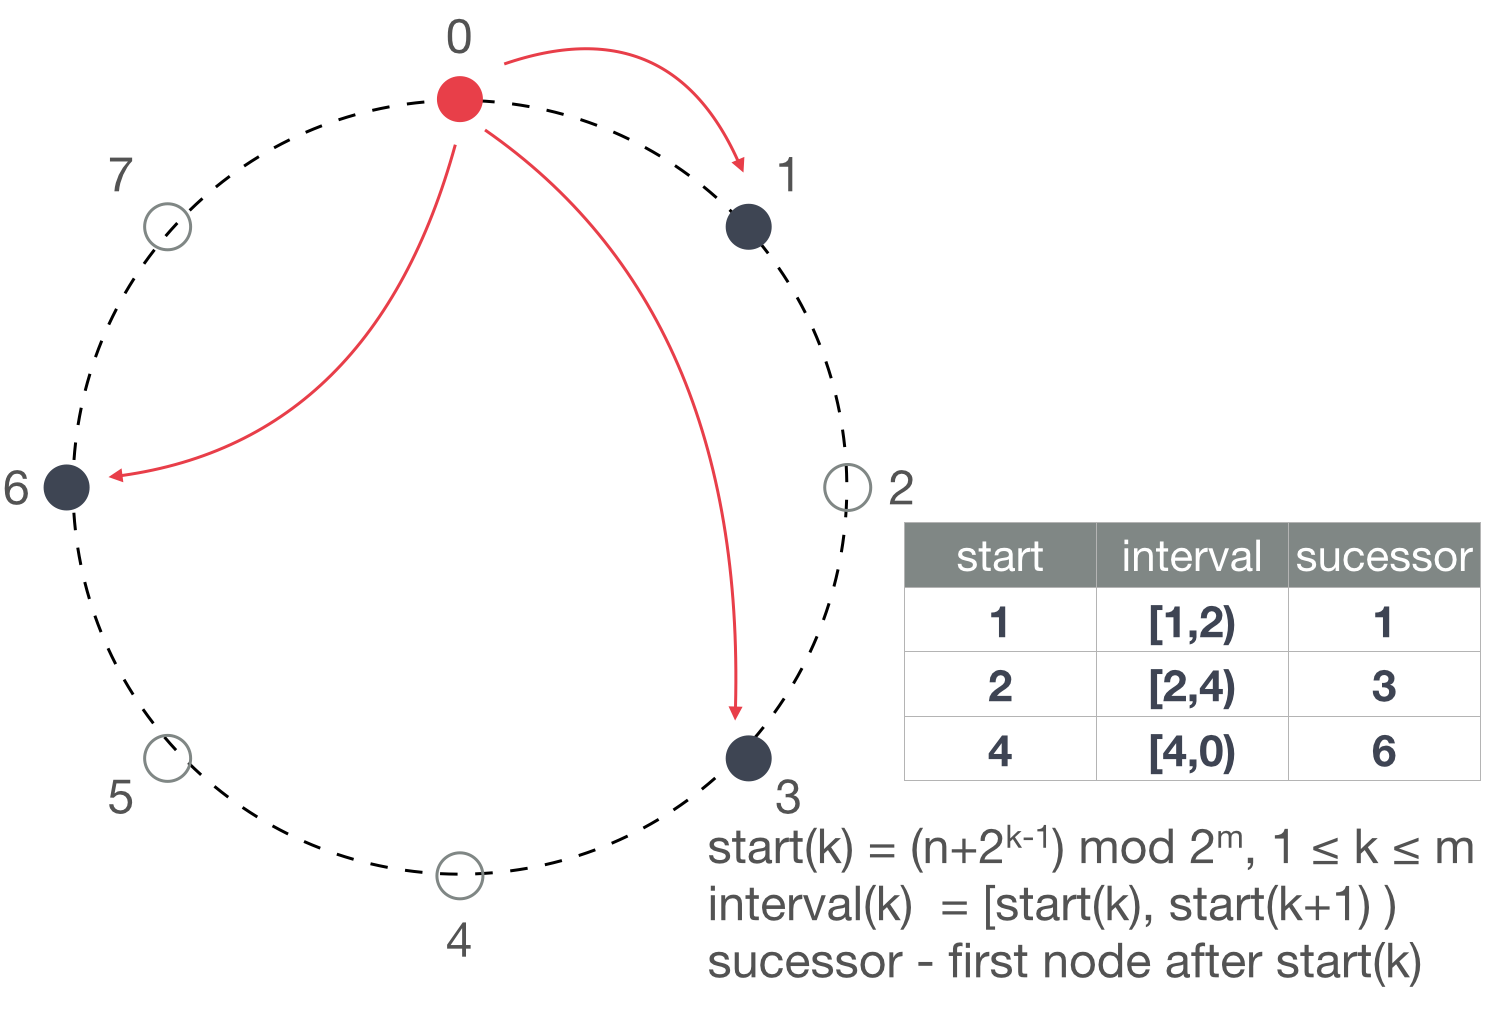
\includegraphics[width=0.2\textwidth]{figs/chord-6}
  \caption{Peer with ID=0 finger table}
  \label{fig:c-6}
\end{figure}

The number of fingers and the fingers we use for a given instance of browserCloud.js are configurable. The reason behind this design decision was that RTCPeerConnections have a significant memory cost, so we have to be considerate in the number of data channels we keep open. In order to give greater flexibility to the developer, we allow the option of picking how many rows of the finger table will be filled by the developer creating a browserCloud.js application. This is also perfect since WebRTC is still a working draft and there might be good developments in resource consumption.

\subsection{Resource Management}

Leveraging the browser's dynamic runtime was a feature we pursue from the beginning of the design for browserCloud.js.

\subsubsection{Job Execution}

A job consists in the partition of tasks which are enriched, with both task code and data, and sent to other peers to be executed. These tasks, which can be represented as functions (job assets), can be defined in runtime, therefore providing a greater flexibility to the developer that is using this system to run the distributed job they want. We can describe the work performed to schedule a job, by the following algorithm:

\begin{itemize}
    \item 1. A user submits a job
    \item 2. The job is divided in smaller computing units, called tasks, each task compromisses of a segment of the data that is going to be processed and the transformation which is going to be applied, that is, a function.
    \item 3. These tasks and data partitions are created
    \item 4. The peer will request the network for other peers availability, the user has the capability to specify how many peers should be used to process this job. This option is given since different jobs might benefit of more or less partition, depending on the data set.
    \item 5. The peer who submitted the job (the peer that is controlled by the user submitting the job) will receive the individual results for each task as they are ready and transmitted. Once all of the results are received, they are aggregated and delivered to the user.
\end{itemize}

\subsection{Architecture of the Software stack}

We can observe a overview of this architecture in Figure~\ref{fig:s-a-n-l}.

\begin{figure}[h!]
  \centering
  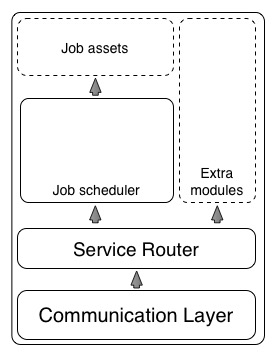
\includegraphics[width=0.2\textwidth]{figs/software-architecture-node-level}
  \caption{Software layers at the peer level}
  \label{fig:s-a-n-l}
\end{figure}


\subsubsection{Communication layer}

The communication layer is responsible for routing messages between peers and establish a connection with the rendezvous point to perform a peer join/leave.

\subsubsection{Service router}

The Service router establishes a protocol for modules like the job scheduler to interact with the network of peers, it uses an event driven model, where modules can register listeners to events that happen on the network or send messages.

\subsubsection{Job scheduler}

The Job scheduler benefits the API of the Service router to implement its logic.

\subsection{API design}

For the user of browserCloud.js, a simple API was created to perform: peer join, message listening and job scheduling as demonstrated by the following code (which should be interpreted as pseudo-code since the API might change with the release of new versions):

\subsubsection{API Usage}

\textit{Peer join}
\begingroup
\scriptsize
\begin{verbatim}
    // browserCloud.js browser module name is called webrtc-explorer.

    var Explorer = require('webrtc-explorer');

    var config = {
        signalingURL: '<signalling server URL>'
    };

    var peer = new Explorer(config);

    peer.events.on('registered', function(data) {
        console.log('registered with Id:', data.peerId);
    });

    peer.events.on('ready', function() {
        console.log('ready to send messages');
    });

    peer.register();
\end{verbatim}
\endgroup

\textit{Listen for messages}
\begingroup
\scriptsize
\begin{verbatim}
    // The only action that has to be performed is listen for the message 
    // event
    peer.events.on('message', function(envelope) {
        console.log(envelope);
    });
\end{verbatim}
\endgroup

\textit{Execute a job}
\begingroup
\scriptsize
\begin{verbatim}
    var browserProcess = require('webrtc-explorer-browser-process');

    var config = {
        signalingURL: 'http://localhost:9000'
    };

    // Make this browser available to execute tasks and also prepared to 
    // issue jobs to the network
    browserProcess.participate(config);

    var start = function() {
        var data = [0,1,2,3,4,5,6,7,8,9,10];  // simple data input
        var task = function(a) {return a+1;}; // e.g of a task (
        var nPeers = 2; // number of peers we are requesting from the network
        // to execute our job

        browserProcess.execute(data, task, nPeers, function done(result) {
            console.log('Received the final result: ', result);
        });
    };
\end{verbatim}
\endgroup

\subsection{Testing framework requirement}

When it comes to testing to test a decentralized browser app or library, the focus stops being how a browser implements a specific behaviour, but how the decentralized network handles node joins and leaves, and whether nodes are effectively communicating between each other. For this scenario, we have a specific set of requirements for the framework, these are:

\begin{itemize}
    \item Have N browsers available, where 1\textless=N\textless=virtually unlimited 
    \item Serve a custom web page for the desired test 
    \item Instruct browsers on demand 
    \item Gather information and evaluate the state as a whole 
\end{itemize}

\subsubsection{browserCloudjs quality test workflow}

In order to evaluate that a browserCloudjs instance is working as desired, we have designed the following workflow, which can also be seen in Figure~\ref{fig:t-f-1}:

\begin{itemize}
    \item 1 - A Web Server is started by the Control Center, this endpoint will be serving the necessary static assets (e,g .html, .css and .js files) that will contain our browserCloudjs module, so that when a browser loads the page through this endpoints, has a way to run browserCloudjs.
    \item 2 - The number of required browsers for the test being executed, are spawned. In our example in Figure~\ref{fig:t-f-1}, we see that number is 2.
    \item 3 - Once the browser loads the web page containing the browserCloudjs module, the Control Center starts sending commands to each browser to execute.
    \item 4 - Since the messages and data transferred between browsers happens in a side channel, browsers report to the Control Center which events were triggered.
    \item 5 - Once all the commands were executed, the Control Center assesses the order in which these events happened and asserts if the behavior was the expected.
\end{itemize}

\begin{figure}[h!]
  \centering
  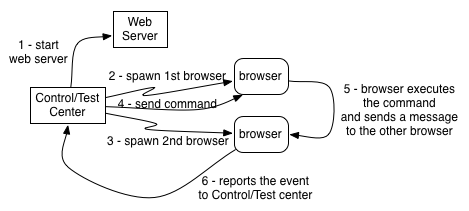
\includegraphics[width=0.4\textwidth]{figs/testing-framework-1}
  \caption{Normal execution of a browserCloudjs test}
  \label{fig:t-f-1}
\end{figure}

\subsubsection{browserCloudjs quality test assessment}

browserCloudjs tests are not linear, a message can be routed between any two browsers through several combinations, depending on the current size of the network and the respective IDs of those browsers, which will influence how their finger table looks like.

In Figure~\ref{fig:t-f-2}, we have an example of two browsers communicating between each other. We can see that some of the browsers between them will have the responsibility to forward the message, while others, will be idle.

\begin{figure}[h!]
  \centering
  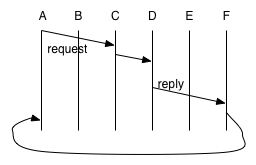
\includegraphics[width=0.2\textwidth]{figs/testing-framework-2}
  \caption{Possible timeline of events for an request from browser A to browser D and the consequent reply}
  \label{fig:t-f-2}
\end{figure}

